\FloatBarrier
\clearpage

\subsection{Likelihood scan results}
\Fig{\ref{fig:ggf_vbf-kl-likelihood-corr-obs}} shows the likelihood scan as a function of \kl.
\Fig{\ref{fig:ggf_vbf-kvv-likelihood-corr-obs}} shows the likelihood scan as a function of \kvv.
Intervals are summarised in \Tab{\ref{table:kl-kvv-likelihood-tab}}.

\begin{figure}[htp]
\centering
	\subfloat[]{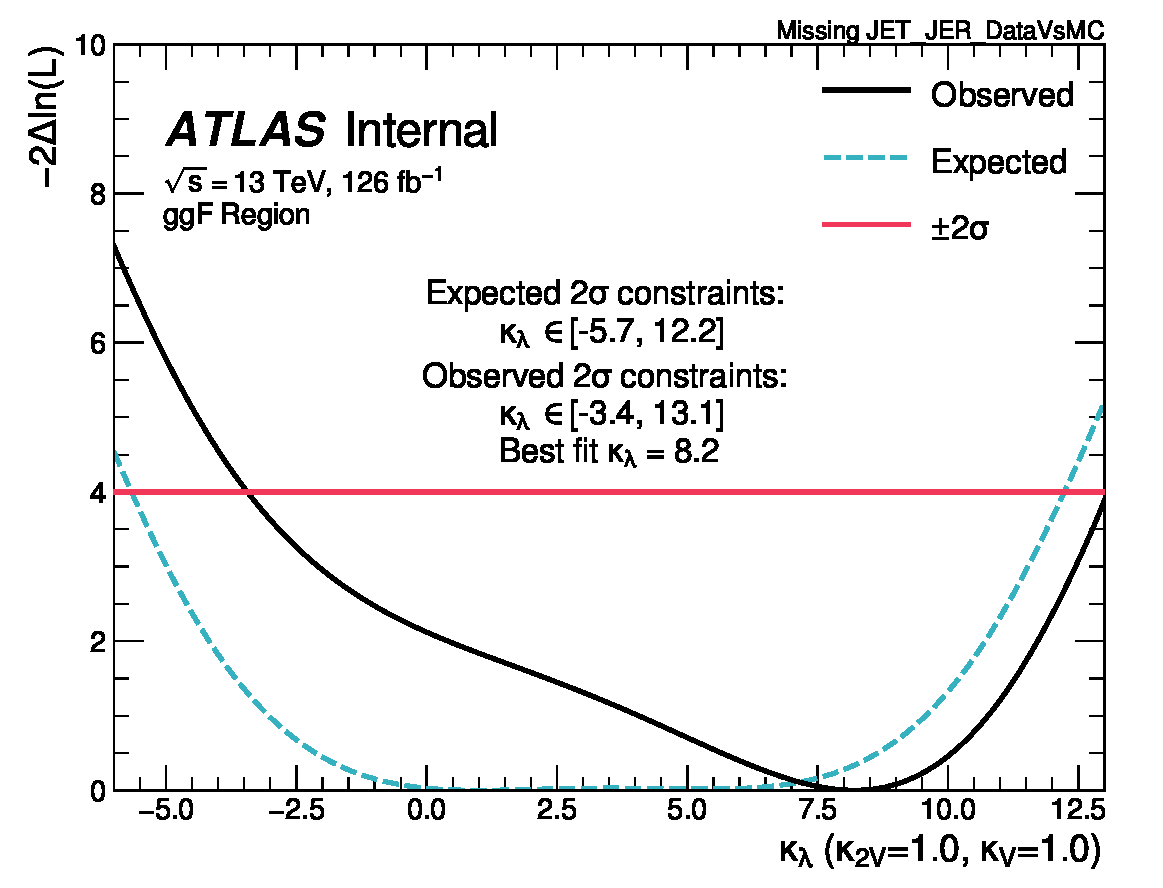
\includegraphics[width=0.45\textwidth]{ggF_kl_9May_logL_scan}}%{\corrscheme/LogLScans25Apr/ggf_kl_asllSys_logL_scan.pdf}}
	\subfloat[]{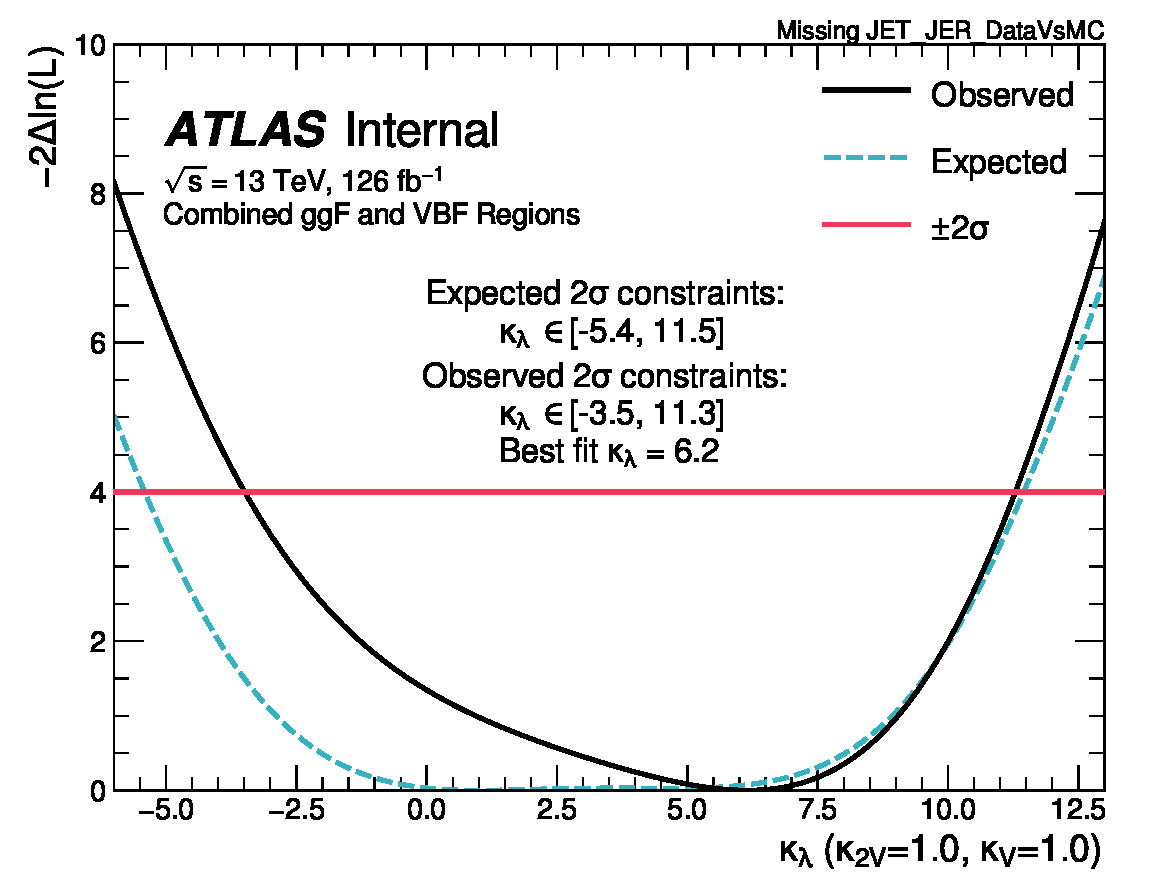
\includegraphics[width=0.45\textwidth]{ggFVBF_kl_9May_logL_scan}}%{\corrscheme/LogLScans25Apr/ggfvbf_kl_allsys_logL_scan.pdf}}
	\caption{Likelihood scan for \kl in ggF only (left) and ggF+VBF combined (right) results.}
	\label{fig:ggf_vbf-kl-likelihood-corr-obs}
\end{figure}

\begin{figure}[htp]
\centering
	\subfloat[]{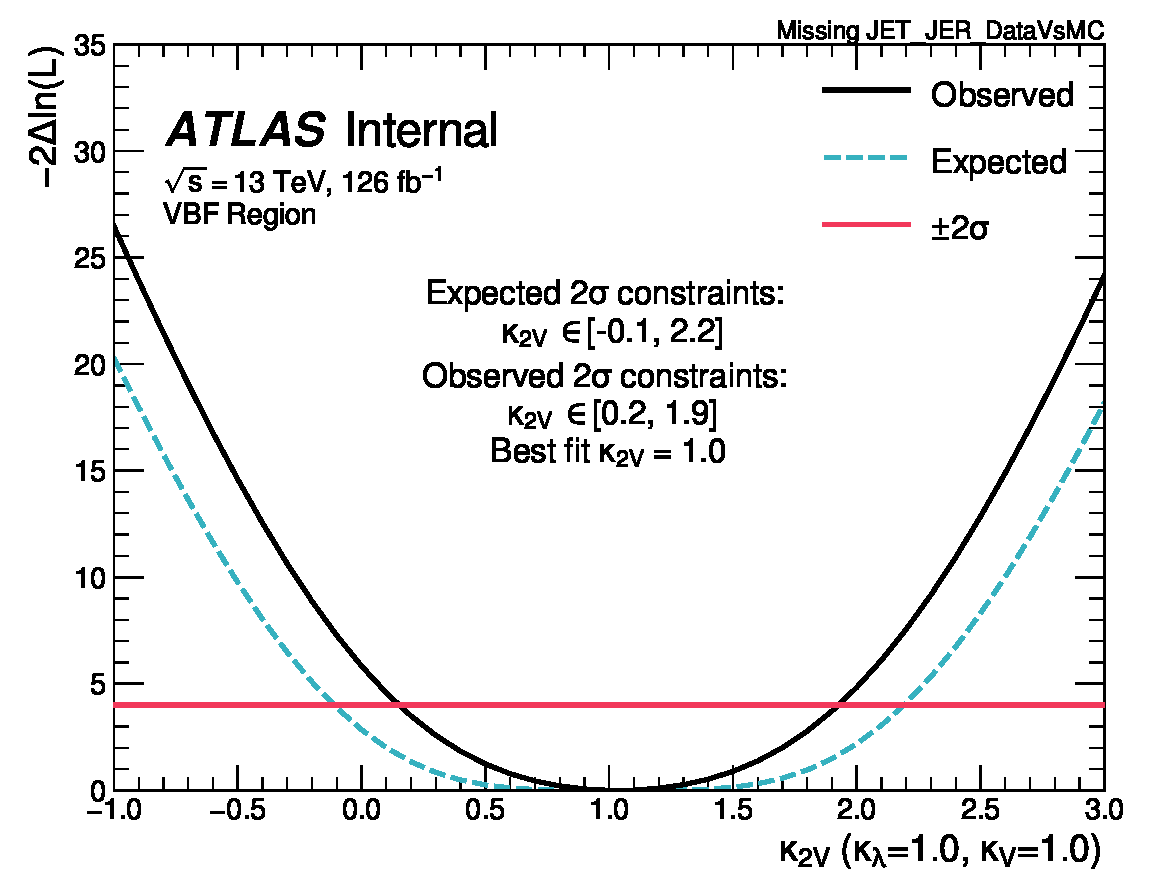
\includegraphics[width=0.45\textwidth]{VBF_k2V_9May_logL_scan}}%{\corrscheme/LogLScans25Apr/VBF_k2v_allSys_logL_scan.pdf}}
	\subfloat[]{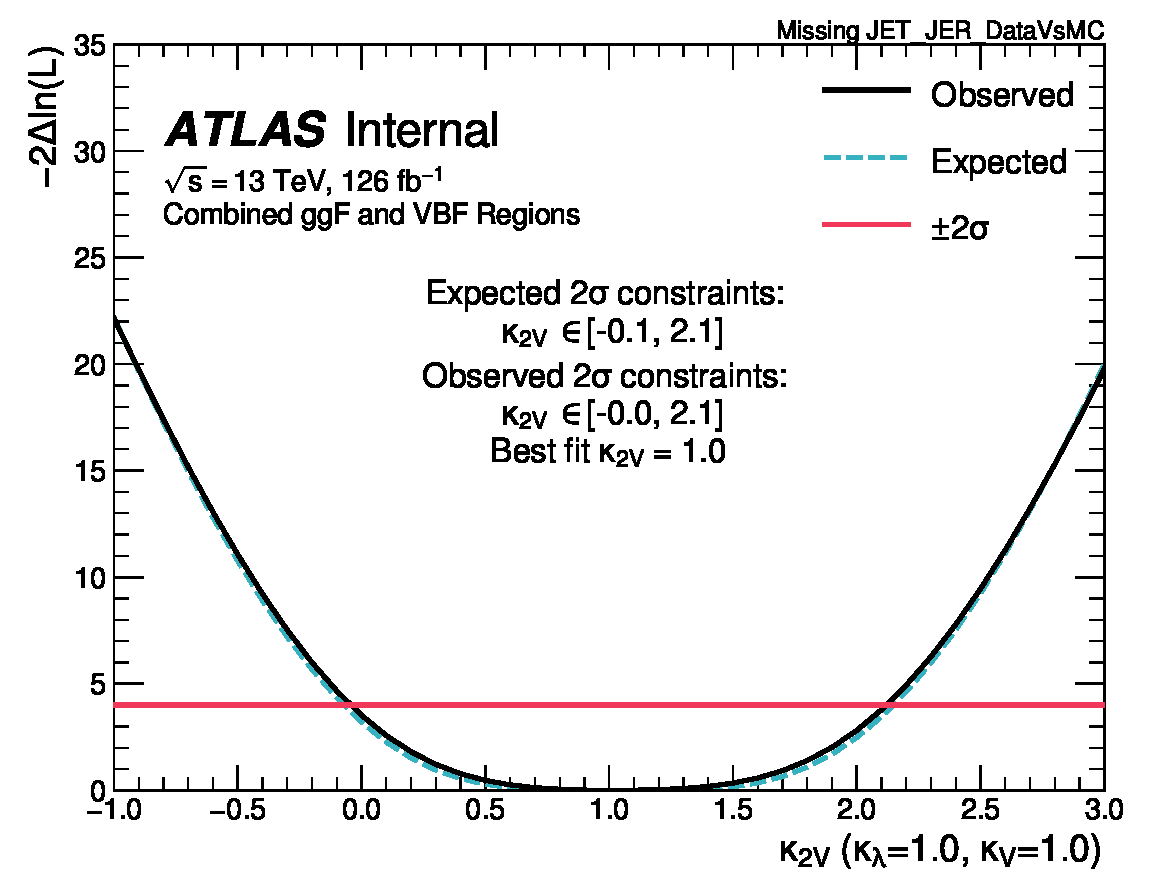
\includegraphics[width=0.45\textwidth]{ggFVBF_k2V_9May_logL_scan}}%{\corrscheme/LogLScans25Apr/ggfvbf_k2v_allsys_logL_scan.pdf}}
	\caption{Likelihood scan for \kvv in VBF only (left) and ggF+VBF combined (right) results.}
	\label{fig:ggf_vbf-kvv-likelihood-corr-obs}
\end{figure}

\begin{table}[h]
	\centering
	\caption{Confidence intervals of \kl and \kvv from likelihood ratio scans.}
	\begin{tabular}{c c c c}
		\toprule
		{Channel} & {Best fit} & {$1\sigma$ Interval Expected} & {$1\sigma$ Interval Observed} \\
		\midrule
		{\kl from ggF only}  & {$8.2$} & {$[-5.7, 12.2]$} & {$[-3.4, 13.1]$} \\
		{\kl from ggF+VBF Channel} & {$6.2$} & {$[-5.4, 11.5]$} & {$[-3.5, 11.3]$} \\
		{\kvv from VBF Channel} & {$1.0$} & {$[-0.1, 2.2]$} & {$[0.2, 1.9]$} \\
		{\kvv from ggF+VBF Channel} & {$1.0$} & {$[-0.1, 2.1]$} & {$[-0.0, 2.1]$} \\
		\bottomrule
	\end{tabular}
\label{table:kl-kvv-likelihood-tab}
\end{table}


\subsection{SMEFT results}
\caveat{This part won't be included in the CONF note but will in the final paper.}
Only the ggF events in the ggF channel is used to derive the SMEFT results showed in this section, namely the contribution from VBF events is neglected.
The 1-D upper limit on the cross section as a function of the five SMEFT parameters are shown in \Fig{\ref{fig:smeft-limit-1d}}.
% Some 2-D contour plots given a pair of the five parameters can be found in \Fig{\ref{fig:smeft-limit-2d}}.
When performing these scans, other parameters are fixed to their SM values (either 1 or 0).

\begin{figure}[h]
	\centering
	\subfloat[]{
		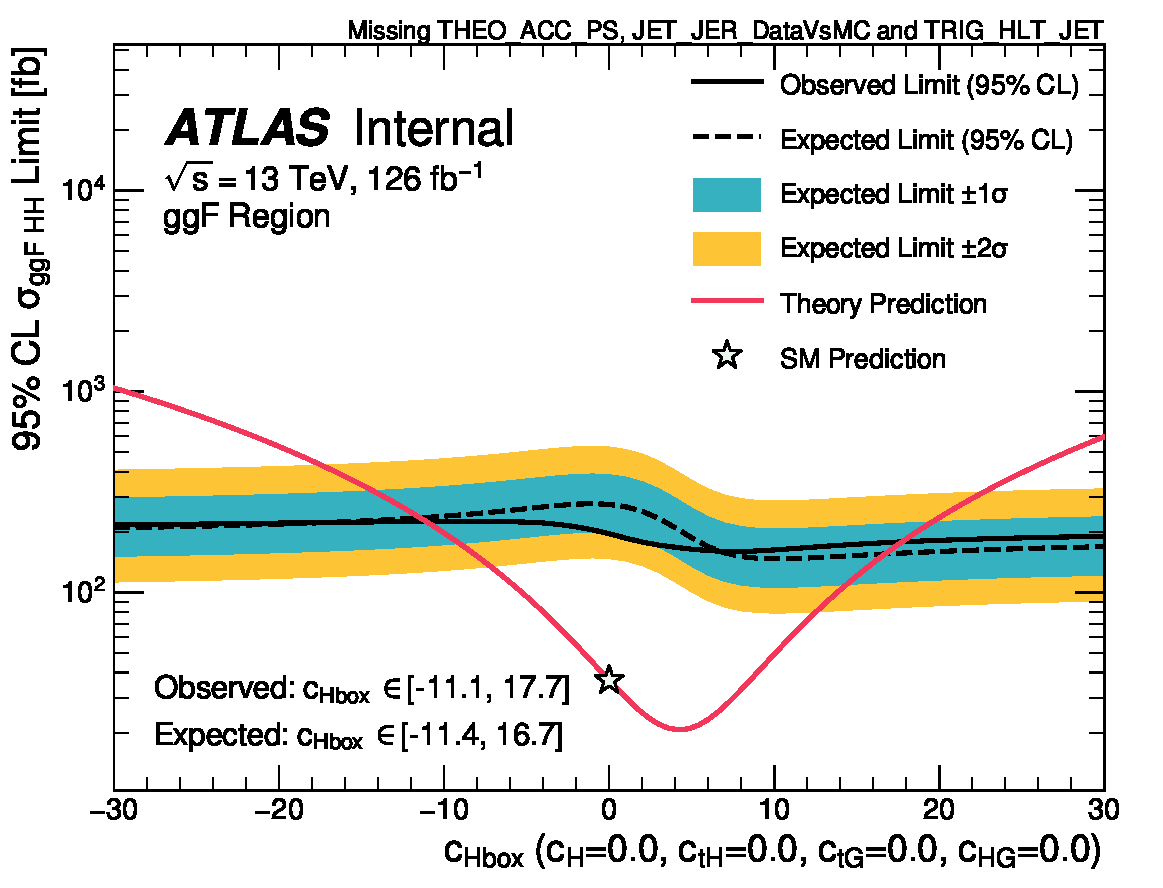
\includegraphics[width=0.33\textwidth]{\corrscheme/limits/smeft_cdp_scan_correlated_fullsyst_unblind_smeft_1dcdp_4b_deta_Xhh_3x2_res_p08_samps_ggf_pd_ggf_161718_mod_cp_0.00_cdp_30.00_ctp_0.00_ctg_0.00_cpg_0.00_cp_0.0_ctp_0.0_ctg_0.0_cpg_0.0_xs.pdf}}
	\subfloat[]{
		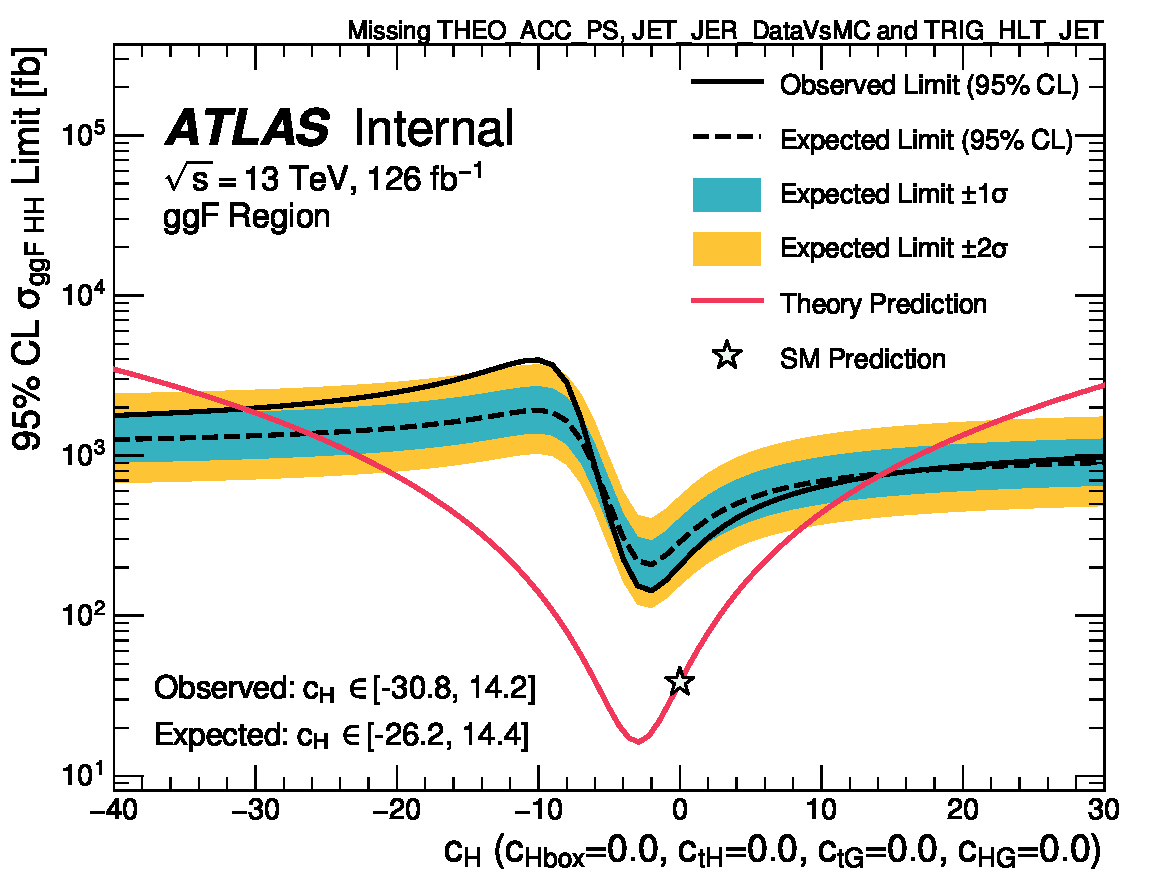
\includegraphics[width=0.33\textwidth]{\corrscheme/limits/smeft_cp_scan_correlated_fullsyst_unblind_smeft_1dcp_4b_deta_Xhh_3x2_res_p08_samps_ggf_pd_ggf_161718_mod_cp_30.00_cdp_0.00_ctp_0.00_ctg_0.00_cpg_0.00_cdp_0.0_ctp_0.0_ctg_0.0_cpg_0.0_xs.pdf}}
	\subfloat[]{
		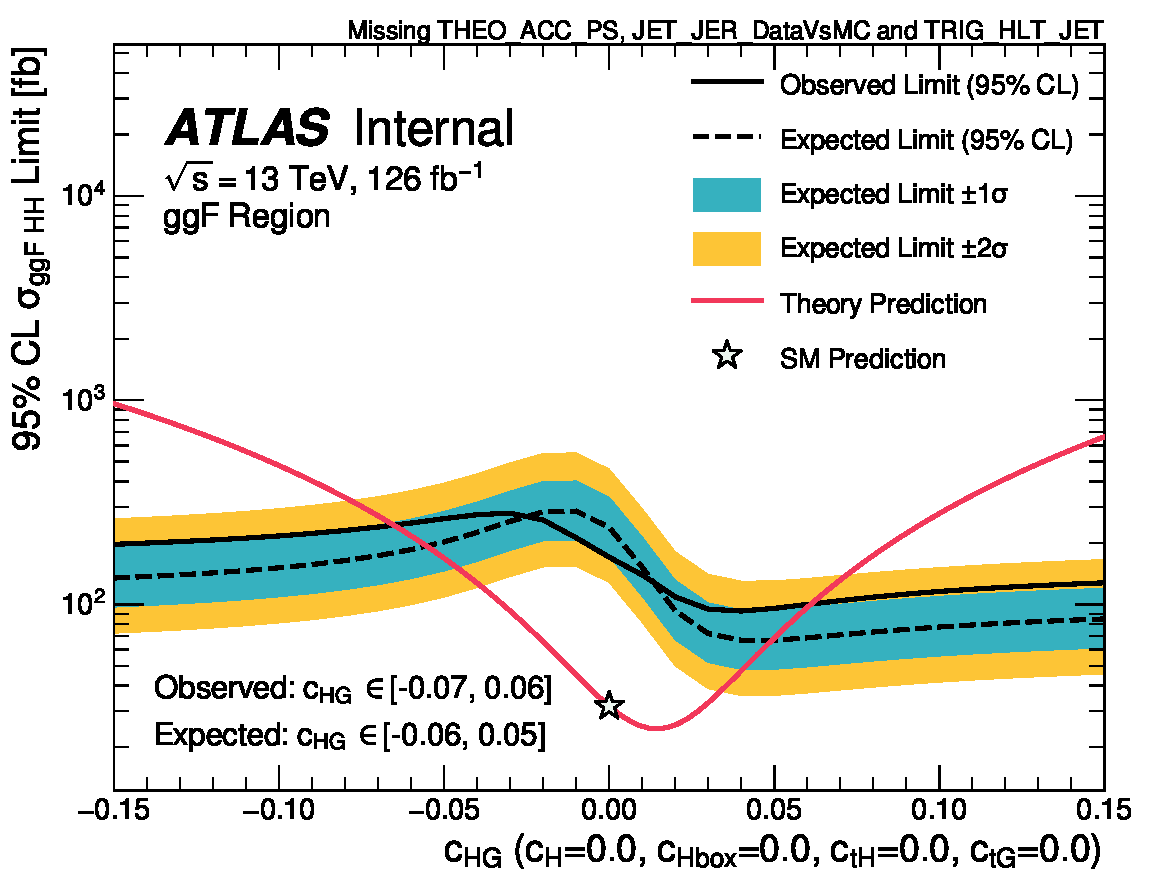
\includegraphics[width=0.33\textwidth]{\corrscheme/limits/smeft_cpg_scan_correlated_fullsyst_unblind_smeft_1dcpg_4b_deta_Xhh_3x2_res_p08_samps_ggf_pd_ggf_161718_mod_cp_0.00_cdp_0.00_ctp_0.00_ctg_0.00_cpg_0.15_cp_0.0_cdp_0.0_ctp_0.0_ctg_0.0_xs.pdf}} \\
	\subfloat[]{
		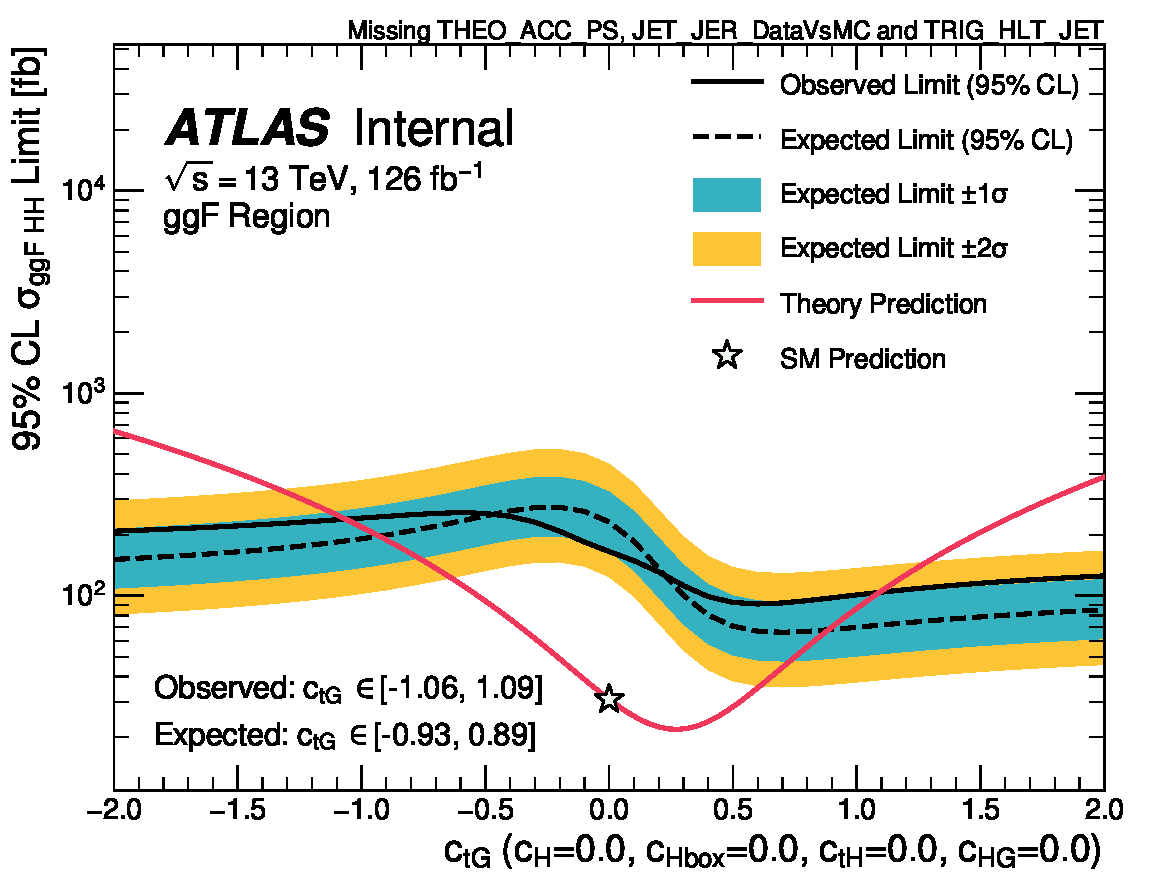
\includegraphics[width=0.33\textwidth]{\corrscheme/limits/smeft_ctg_scan_correlated_fullsyst_unblind_smeft_1dctg_4b_deta_Xhh_3x2_res_p08_samps_ggf_pd_ggf_161718_mod_cp_0.00_cdp_0.00_ctp_0.00_ctg_2.00_cpg_0.00_cp_0.0_cdp_0.0_ctp_0.0_cpg_0.0_xs.pdf}}
	\subfloat[]{
		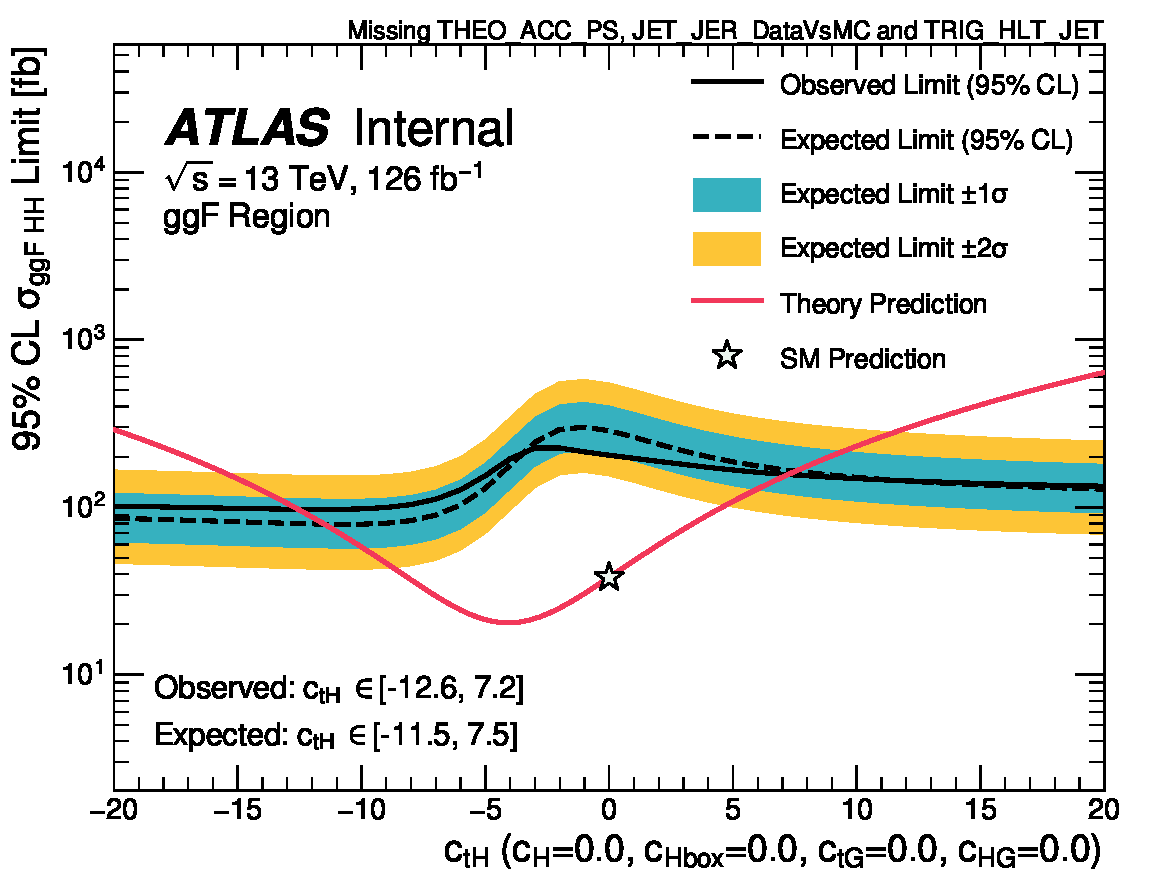
\includegraphics[width=0.33\textwidth]{\corrscheme/limits/smeft_ctp_scan_correlated_fullsyst_unblind_smeft_1dctp_4b_deta_Xhh_3x2_res_p08_samps_ggf_pd_ggf_161718_mod_cp_0.00_cdp_0.00_ctp_20.00_ctg_0.00_cpg_0.00_cp_0.0_cdp_0.0_ctg_0.0_cpg_0.0_xs.pdf}}
	\caption{1D limit for the five SMEFT parameters.
	Other parameters are set to their SM predictions.
	}
	\label{fig:smeft-limit-1d}
\end{figure}

% \begin{figure}[h]
% 	\centering
% 	\subfloat[]{
% 		\includegraphics[width=0.45\textwidth]{\corrscheme/limits/smeft_2D_scan_correlated_fullsyst_unblind_smeft_2dcdp_4b_deta_Xhh_3x2_res_p08_samps_ggf_pd_ggf_161718_ctp0.0_exclusion.pdf}}
% 	\subfloat[]{
% 		\includegraphics[width=0.45\textwidth]{\corrscheme/limits/smeft_2D_scan_correlated_fullsyst_unblind_smeft_2dcpg_4b_deta_Xhh_3x2_res_p08_samps_ggf_pd_ggf_161718_cdp0.0_exclusion.pdf}} \\
% 	\subfloat[]{
% 		\includegraphics[width=0.45\textwidth]{\corrscheme/limits/smeft_2D_scan_correlated_fullsyst_unblind_smeft_2dctg_4b_deta_Xhh_3x2_res_p08_samps_ggf_pd_ggf_161718_cdp0.0_exclusion.pdf}}
% 	\subfloat[]{
% 		\includegraphics[width=0.45\textwidth]{\corrscheme/limits/smeft_2D_scan_correlated_fullsyst_unblind_smeft_2dctp_4b_deta_Xhh_3x2_res_p08_samps_ggf_pd_ggf_161718_cdp0.0_exclusion.pdf}}
% 	\caption{Selected 2D limit contours for the five SMEFT parameters.
% 	Other parameters are set to their SM predictions.}
% 	\label{fig:smeft-limit-2d}
% \end{figure}

\FloatBarrier
\clearpage

